\documentclass[12pt,a4paper]{article}

% ---------- BASIC PACKAGES ----------
\usepackage[utf8]{inputenc}        % Encoding
\usepackage[T1]{fontenc}           % Font encoding
\usepackage[english]{babel}        % Language
\usepackage{lmodern}               % Improved font rendering
\usepackage{microtype}             % Better spacing and typography
\usepackage[a4paper,margin=1in]{geometry}  % Page setup

% ---------- MATH PACKAGES ----------
\usepackage{amsmath}               % Core math features
\usepackage{amssymb}               % More symbols
\usepackage{amsthm}                % Theorems, lemmas, proofs
\usepackage{mathtools}             % Enhancements to amsmath
\usepackage{bm}                    % Bold math symbols
\usepackage{physics}               % Derivatives, vectors, etc.
\usepackage{esdiff}                % Alternative differential notation
\usepackage{cancel}                % Cancel terms in equations
\usepackage{mathrsfs}              % Script fonts
\usepackage{dsfont}                % Double stroke fonts (e.g. indicator function)
\usepackage{leftidx}               % Left side equation numbering

% ---------- THEOREM ENVIRONMENTS ----------
\theoremstyle{plain}
\newtheorem{theorem}{Theorem}[section]
\newtheorem{lemma}[theorem]{Lemma}
\newtheorem{proposition}[theorem]{Proposition}
\newtheorem{corollary}[theorem]{Corollary}

\theoremstyle{definition}
\newtheorem{definition}[theorem]{Definition}
\newtheorem{example}[theorem]{Example}

\theoremstyle{remark}
\newtheorem{remark}[theorem]{Remark}

% ---------- INLINE NOTE ENVIRONMENT ----------
\usepackage{xparse}

\newcounter{note}
\renewcommand{\thenote}{\arabic{note}} % Numbering style (1, 2, 3, ...)

\NewDocumentEnvironment{note}{} % no arguments now
{
    \par\scriptsize% smaller text (adjust as desired)
    \refstepcounter{note}%
    \noindent\textbf{Note~\thenote.}~%
    \ignorespaces
}
{
    \par\normalsize\ignorespacesafterend
}

% ---------- CUSTOM SHORTCUTS ----------
\newcommand{\R}{\mathbb{R}}
\newcommand{\N}{\mathbb{N}}
\newcommand{\Z}{\mathbb{Z}}
\newcommand{\Q}{\mathbb{Q}}
\newcommand{\C}{\mathbb{C}}
\newcommand{\eps}{\varepsilon}
\newcommand{\del}{\partial}
\newcommand{\E}{\mathbb{E}}
\newcommand{\Var}{\mathrm{Var}}
\newcommand{\Cov}{\mathrm{Cov}}
\newcommand{\defeq}{\vcentcolon=}
\DeclareMathOperator*{\argmin}{arg\,min}

% ---------- FIGURES & TABLES ----------
\usepackage{graphicx}              % Include images
\usepackage{float}                 % Better control of figure placement
\usepackage{caption}               % Better captions
\usepackage{subcaption}            % Subfigures
\usepackage{booktabs}              % Nicer tables
\usepackage{multirow}              % Multi-row cells in tables

% ---------- REFERENCES & LINKS ----------
\usepackage[hidelinks]{hyperref}   % Clickable refs
\usepackage{cleveref}              % Smart cross-referencing
\usepackage[numbers,sort&compress]{natbib} % Bibliography style (optional)

% ---------- COLORS & MISC ----------
\usepackage{xcolor}                % Colored text
\usepackage{enumitem}              % Custom lists
\usepackage{tcolorbox}             % Colored boxes for highlighting
\usepackage{tikz}                  % Draw diagrams
\usepackage{tikz-cd}               % Commutative diagrams

% ---------- DOCUMENT START ----------
\title{MIT Cheetah 3 Architecture}
\author{Raahim Hashmi}
\date{\today}

\begin{document}

\maketitle

\section{Introduction}
This document contains an in-depth explanation of MIT Cheetah 3's architecture (see note \ref{note:state-estimation}). The modules are taken from the diagram below: 
\begin{note}
    For now, I am not including discussion on the state estimation module. Any module that requires the robot's current state is either obtained through state estimation, or in the case of convex MPC, is a function of the previous state and control inputs.
    \label{note:state-estimation}
\end{note}
\begin{figure}[H]
    \centering
    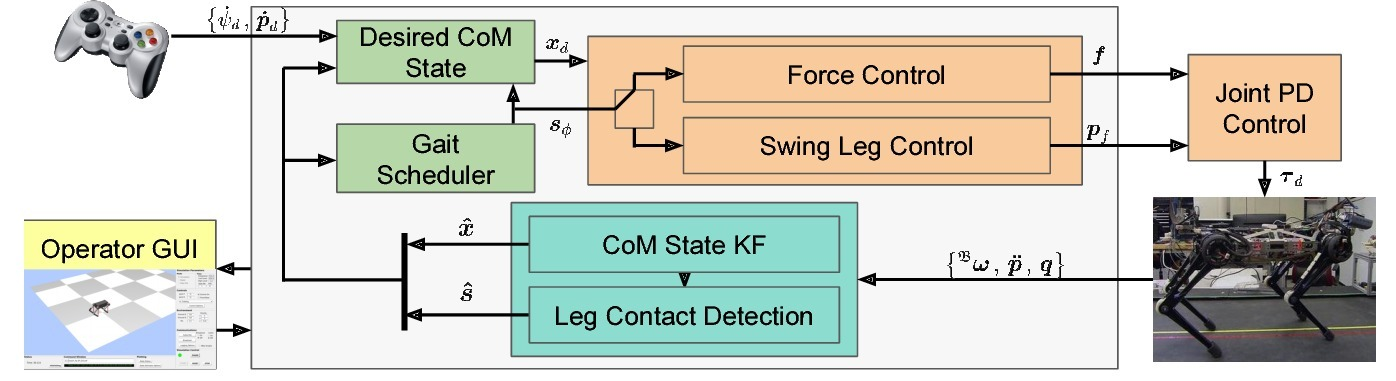
\includegraphics[width=\linewidth]{diagram.jpg}
    \caption{Architecture diagram from the MIT Cheetah 3 paper. The green block is the higher-level planner, the orange block is the leg and body controller, and the cyan block is the state estimation module.}
    \label{fig:diagram}
\end{figure}

\section{Architecture}

In this section, all explicitly defined modules (except for state estimation) as well as their implicit submodules will be detailed. Each module and submodule will be given a unique identifier that consists of a name and a signature that indicates its inputs and outputs. For example, a module with 3 inputs and 2 outputs would be identified as: \[\texttt{Module-Name}(input_1, input_2, input_3 \rightarrow output_1, output_2)\]

\subsection{User Commands}

The user commands are the highest level input to the entire architecture. The user sets a desired angular velocity $\mathbf{\dot{\psi}}_d = \begin{bmatrix} 0 \\ 0 \\ \dot{\psi_z}_d \end{bmatrix}$ and a desired linear velocity $\mathbf{\dot{p}}_{c,d} =  \begin{bmatrix} \dot{p_x}_{c,d} \\ \dot{p_y}_{c,d} \\ 0 \end{bmatrix}$ for the robot's center of mass (CoM). \[\texttt{Commands}(\rightarrow \mathbf{\dot{\psi}}_d, \mathbf{\dot{p}}_{c,d})\]

\subsection{Gait Scheduler}

The gait scheduler is responsible for determining the stance and swing legs based on a gait schedule. The authors use a position-based feedback approach to determine unexpected contacts, denoted by $\hat{s}_i \in \{ 0 = \text{leg i has not made contact}, 1 = \text{leg i made contact} \}$. The gait scheduler takes the estimated contacts as inputs and outputs $s_{\phi_i} \in \{0 = \text{leg i is in swing}, 1 = \text{leg i is in stance}\}$ for $i \in \{1, 2, 3, 4\}$ where $\phi_i \in [0, 1)$ is a phase variable that cycles over a defined period and is used to differentiate between swing and stance phases for leg $i$ based on a defined range. It is calculated as 
\[\phi_i = \dfrac{t - t_0}{T} - \gamma_i\] 
where $t$ is the current time, $t_0$ is the start time of the current gait cycle, $T$ is the total duration of the gait cycle, and $\gamma_i$ is an offset that defines the phase relationship between legs as seen in figure \ref{fig:gait}.
\begin{figure}[H]
    \centering
    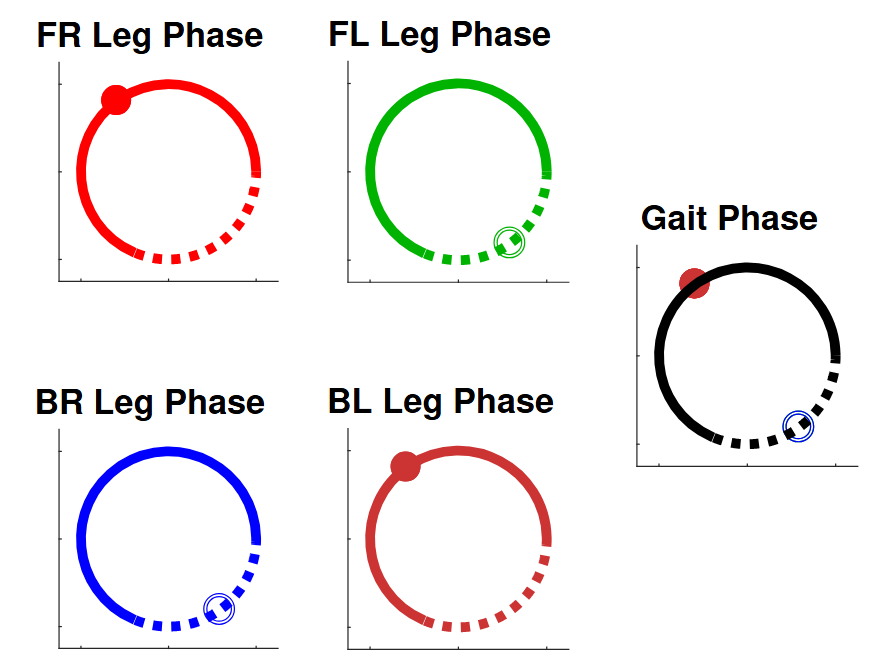
\includegraphics[width=0.6\linewidth]{gait.png}
    \caption{Gait scheduler diagram from the MIT Cheetah 3 paper. The phase variable $\phi_i$ is used to determine the swing and stance legs based on a defined gait schedule. The solid line indicates the stance phase while the dashed line indicates the swing phase. The solid and hollow circles indicate the predefined offset $\gamma_i$ for each leg.}
    \label{fig:gait}
\end{figure}
However, we do not want to work with purely time based scheduling, given that we have $\hat{s}_i$. The authors use the underlying time based schedule to make an event-based FSM (shown in figure \ref{fig:fsm}) that has each leg go through the swing phase normally but when it makes contact, it attempts to maintain that position and after some delay, it transitions to stance phase. 

\begin{figure}[H]
    \centering
    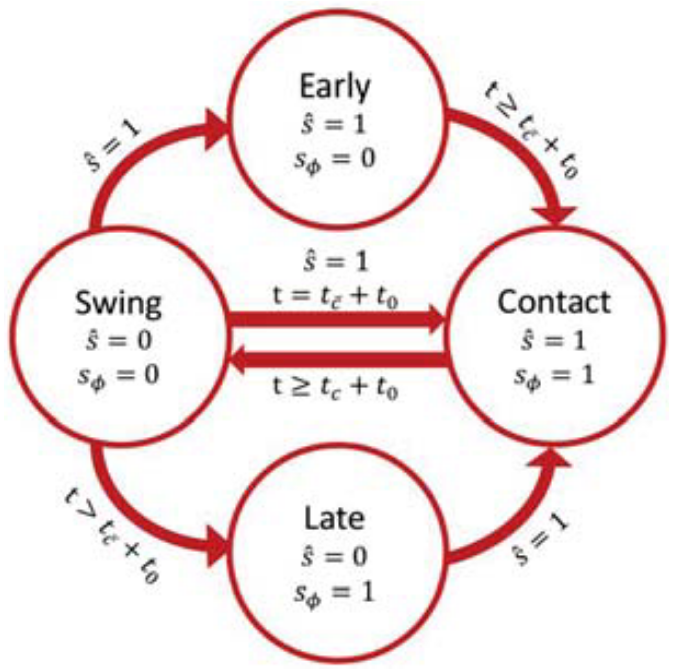
\includegraphics[width=0.4\linewidth, height=0.4\linewidth]{fsm.png}
    \caption{Event-based FSM for gait scheduling. The leg transitions to stance phase upon making contact, and after a delay, it transitions back to swing phase.}
    \label{fig:fsm}
\end{figure}

\[\texttt{Gait-Scheduler}(\hat{s}_i \rightarrow s_{\phi_i})\]

\subsection{Desired CoM State}

Based on the user commands and the gait schedule, the desired CoM state is computed as the CoM of a predictive virtual support polygon estimated using the foot positions $\mathbf{p}_i$ and the gait schedule to determine the desired CoM position $\mathbf{p}_{c,d}$.

For each leg $i$, $\Phi_i$ represents the total weighting factor for the foot - the closer the leg $i$ is to the middle of the stance phase, the more dependable it is and $\Phi_i$ is higher. 
\[ \Phi_i = s_{\phi_i}K_{c_{\phi_i}} + \bar{s}_{\phi_i}K_{\bar{c}_{\phi_i}}\]
where
\[K_{c_{\phi_i}} = \dfrac{1}{2}\big[\erf(\frac{\phi_i}{\sigma_{c_0}\sqrt{2}}) + \erf(\frac{1 - \phi_i}{\sigma_{c_0}\sqrt{2}})\big]\]
\[K_{\bar{c}_{\phi_i}} = \dfrac{1}{2}\big[2 + \erf(\frac{-\phi_i}{\sigma_{\bar{c}_0}\sqrt{2}}) + \erf(\frac{\phi_i-1}{\sigma_{\bar{c}_0}\sqrt{2}})\big]\]
For each leg, two virtual points, $\mathbf{\xi}^-_i$ and $\mathbf{\xi}^+_i$ are defined, that represent the predicted relative availability of each leg as compared to its adjacent legs. 
\[
\begin{bmatrix}
    \mathbf{\xi}^-_i \\[4pt]
    \mathbf{\xi}^+_i
\end{bmatrix} = \begin{bmatrix}
    \mathbf{p}_i & \mathbf{p}^-_i\\[4pt]
    \mathbf{p}_i & \mathbf{p}^+_i
\end{bmatrix} 
\begin{bmatrix}
    \Phi_i \\[4pt]
    1 - \Phi_i
\end{bmatrix}\]
where $\mathbf{p}^-_i$ and $\mathbf{p}^+_i$ are the positions of the legs adjacent to leg $i$ in the clockwise and counterclockwise directions, respectively. Using these virtual points, the predictive support polygon vertex contributed by leg $i$ can be computed as 
\[ \mathbf{\xi}_i = \dfrac{\Phi_i\mathbf{p}_i + \Phi_{i^-}\mathbf{\xi}^-_{i} + \Phi_{i^+}\mathbf{\xi}^+_{i}}{\Phi_i + \Phi_{i^-} + \Phi_{i^+}}\]

The desired CoM is then computed as the mean of the vertices of the predictive support polygon:
\[ \mathbf{p}_{c,d} = \dfrac{1}{4}\sum_{i=1}^{4} \mathbf{\xi}_i\]

\[\texttt{Desired-CoM}(\mathbf{p}_i, \phi_i, s_{\phi_i} \rightarrow \mathbf{p}_{c,d})\]

\begin{figure}[H]
    \centering
    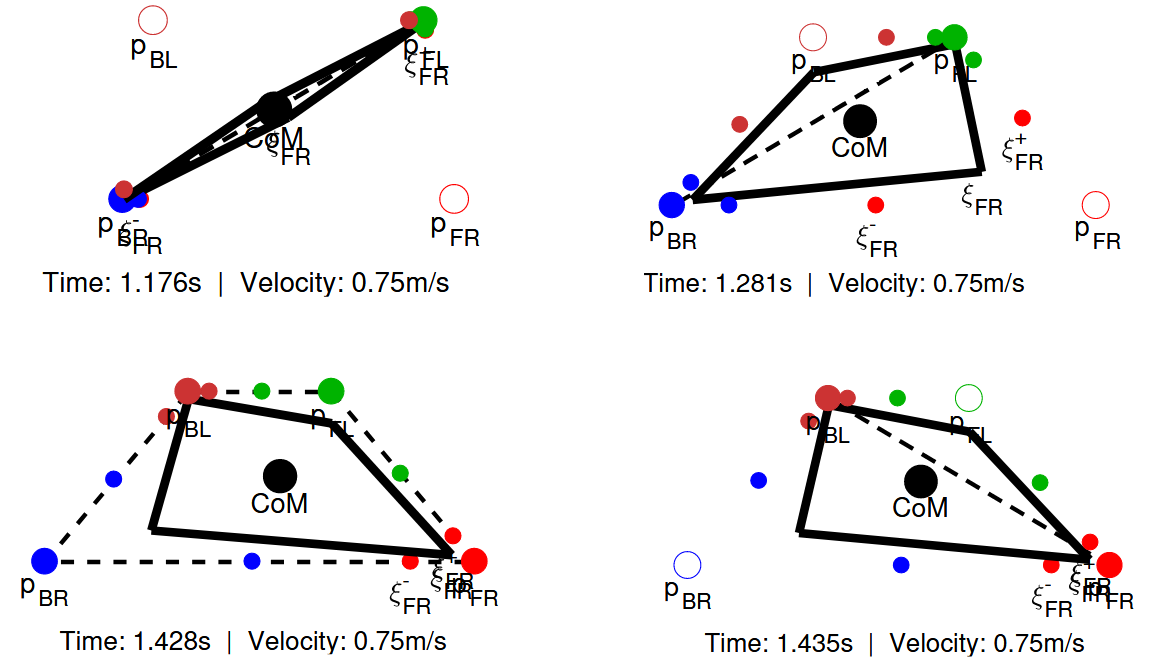
\includegraphics[width=0.6\linewidth]{polygon.png}
    \caption{How the predictive support polygon (solid black) evolves based on the gait schedule. The CoM shifts from the instantaneous support line (dashed black) towards the legs that are closer to the ground (solid circles)}
\end{figure}

\subsection{Force Control}

To balance the robot and track a desired CoM state, a controller is used to optimize the ground reaction forces (GRFs) at each foot. It takes in the foot positions $\mathbf{p}_i$ and the state $\mathbf{x}$ of the CoM of the robot, comprising of the CoM position $\mathbf{p}_c$, CoM velocity $\mathbf{\dot{p}}_c$, orientation $\mathbf{\psi}$, and angular velocity $\mathbf{\dot{\psi}}$, the desired state $\mathbf{x}_d$, and the gait schedule, and outputs the desired GRFs $\mathbf{F}^*$ for each foot.

\[\texttt{Force-Control}{(s_{\phi_i}, \mathbf{p}_i, \mathbf{x}, \mathbf{x}_d \rightarrow \mathbf{F}^*)}\]

\begin{note}
    Need to look into what solvers can be used for the upcoming optimization problems - the authors discuss ECOS and qpOASES. 
\end{note}

There are two methods of force control - Balance Controller and Convex Model Predictive Control (MPC) - discussed by the authors, with any one being used for the robot at a time.

\subsubsection{Balance Controller}

The balance controller enforces PD control on the CoM of the robot. Due to the structure of the robot, the authors make an approximation of the foward dynamics model that relates the GRFs to the CoM forces and torques:
\begin{equation}
    \underbrace{\begin{bmatrix}
        \mathbf{I}_3 & \cdots & \mathbf{I}_3 \\
        \left[\mathbf{p}_1 - \mathbf{p}_c\right]_\times & \cdots & \left[\mathbf{p}_4 - \mathbf{p}_c\right]_\times
    \end{bmatrix}}_{\mathbf{A}}
\mathbf{F}
=
\underbrace{\begin{bmatrix}
    m(\ddot{\mathbf{p}}_c + \mathbf{g}) \\[4pt]
    \mathbf{I_G} \mathbf{\dot{\psi}}
\end{bmatrix}}_{\mathbf{b}}
\end{equation}
where $\mathbf{I}_3$ is the $3 \times 3$ identity matrix, $\left[\mathbf{p}_i - \mathbf{p}_c\right]_\times$ is defined as the skew-symmetric matrix such that $(\mathbf{p}_i - \mathbf{p}_c) \times \mathbf{v} = \left[\mathbf{p}_i - \mathbf{p}_c\right]_\times \mathbf{v}$ for any vector $\mathbf{v}$, $m$ is the mass of the robot, $\ddot{\mathbf{p}}_c$ is the CoM acceleration, $\mathbf{g}$ is the gravitational acceleration, $\mathbf{I_G}$ is the centroidal rotational inertia matrix, and $\mathbf{\dot{\psi}}$ is the CoM angular velocity. 

The PD control law to compute the desired CoM acceleration $\ddot{\mathbf{p}}_{c,d}$ and CoM angular velocity $\dot{\psi}_d$ is given as:
\[
\begin{bmatrix}
    \mathbf{\ddot{p}}_{c,d} \\[4pt]
    \mathbf{\dot{\psi}}_d
\end{bmatrix} = 
\begin{bmatrix}
    \mathbf{K}_{p,p}(\mathbf{p}_{c,d} - \mathbf{p}_c) + \mathbf{K}_{d,p}(\mathbf{\dot{p}}_{c,d} - \mathbf{\dot{p}}_c) \\[4pt]
    \mathbf{K}_{p,\psi}\log({\mathbf{R}_{\psi_d}\mathbf{R}_\psi^T}) + \mathbf{K}_{d,\psi}(\mathbf{\dot{\psi}}_d - \mathbf{\dot{\psi}})
\end{bmatrix}
\]
where $\mathbf{K}_{p,p}$ and $\mathbf{K}_{d,p}$ are the position and velocity PD gain matrices, $\mathbf{K}_{p,\psi}$ and $\mathbf{K}_{d,\psi}$ are the orientation and angular velocity PD gain matrices, $\mathbf{R}_{\psi_d}$ represents the desired orientation as a rotation matrix, and $\mathbf{R}_\psi$ represents the current orientation as a rotation matrix. For all $\mathbf{R} \in SO(3)$, $\mathbf{R}$ can be diagonalized as $\mathbf{R} = \mathbf{PDP}^{-1}$. The logarithm of $\mathbf{R}$, denoted as $\log(\mathbf{R})$, can then be defined as $\log(\mathbf{R}) = \mathbf{PD}'\mathbf{P}^{-1}$, where $\mathbf{D}'_{ii} = \log(\mathbf{D}_{ii})$ (see note \ref{note:dimension}).
% To obtain the difference in orientations about more than one axis, simply computing the difference between the angles about each axis does not work as it does not account for the non-commutativity of such rotations. A method to compute the difference is to use the logarithmic map from $SO(3)$ to its Lie algebra $\mathfrak{so}(3)$ and compute the magnitude of the difference there. This can be done by computing $\log({\mathbf{R}_{\psi_d}\mathbf{R}_\psi^T})$ which gives the difference in orientations as a skew-symmetric matrix in $\mathfrak{so}(3)$ whose Frobenius norm gives the geodesic distance between the two rotations on the manifold defined by $SO(3)$.
\begin{note}
I am unable to reconcile how the dimensions match up in the expression for $\dot{\psi}_d$ - specifically, $\mathbf{K}_{p,\psi}\log({\mathbf{R}_{\psi_d}\mathbf{R}_\psi^T}) \in \mathbb{R}^{3 \times 3}$ and $\mathbf{K}_{d,\psi}(\dot{\psi}_d - \dot{\psi}) \in \mathbb{R}^3$, so their sum isn't defined, and by checking the dimensions of $\mathbf{b}$, we know $\mathbf{b} \in \mathbb{R}^3$. My guess is that it should be $\| \log({\mathbf{R}_{\psi_d}\mathbf{R}_\psi^T}) \|_F$, the Frobenius norm of the matrix which corresponds to the geodesic distance between the rotations $\psi_d$ and $\psi$ on the manifold defined by $SO(3)$. As this would be a scalar, so accordingly $\mathbf{K}_{p,\psi}$ should be a $3 \times 1$ vector.
\label{note:dimension}
\end{note}

The desired CoM forces and torques are then computed as:
\[
\mathbf{b}_d =
\begin{bmatrix}
m(\mathbf{\ddot{p}}_{c,d} + \mathbf{g}) \\[4pt]
\mathbf{I_G} \mathbf{\dot{\psi}}_d
\end{bmatrix}
\]

As $\mathbf{A}$ is not invertible in equation (1), a numerical solution, such as least squares, can be used to compute the GRFs $\mathbf{F}^*$ corresponding to $\mathbf{b}_d$. However, there are other considerations as well, such as the total force being exerted $\|\mathbf{F}\|$ and the deviation from the GRFs at the previous time step $\mathbf{F}^*_{\text{prev}}$. As such, the authors formulate the following quadratic program (QP) to compute the optimal GRFs $\mathbf{F}^*$:
\[
\mathbf{F}^* = 
\argmin_{\mathbf{F} \in \mathbb{R}^{12}}
    (\mathbf{A}\mathbf{F} - \mathbf{b}_d)^{T} \mathbf{S} (\mathbf{A}\mathbf{F} - \mathbf{b}_d)
    + \alpha \|\mathbf{F}\|^2 
    + \beta \|\mathbf{F} - \mathbf{F}_{\text{prev}}^*\|^2
\quad
\text{s.t.} \quad
\mathbf{C}\mathbf{F} \leq \mathbf{d}
\]
where $\mathbf{S}, \alpha, \beta$ are weight matrices/scalars. The constraint $\mathbf{C}\mathbf{F} \leq \mathbf{d}$ ensures the GRFs remain with the friction pyramid and that normal forces are within feasible bounds which switch between support-leg and swing-leg bounds based on the scheduled contact $s_{\phi_i}$.

\subsubsection{Convex Model Predictive Control}

Model Predictive Control (MPC) is a common approach used in robotics for determining controls that are optimal over a finite time horizon (see note \ref{note:mpc}). The authors make approximations of their robot's dynamics to enable the following optimization problem to be convex:
\[
\mathbf{F}^* = \argmin_{\mathbf{F}_{1:k}} \sum_{i=1}^{k} 
    (\mathbf{x}_i - \mathbf{x}_i^{\text{ref}})^T 
    \mathbf{Q}_i 
    (\mathbf{x}_i - \mathbf{x}_i^{\text{ref}})
    + 
    \mathbf{F}_i^T
    \mathbf{R}_i 
    \mathbf{F}_i
\]
where $k$ is the time horizon, $\mathbf{x}_i$ is the state of the robot at the time step $i$, $\mathbf{x}_i^{\text{ref}}$ is the reference state at time step $i$, $\mathbf{F}_i$ is the control input at time step $i$, and $\mathbf{Q}_i, \mathbf{R}_i$ are weight matrices. The authors approximate $\mathbf{x}_i$ as a linear function of the previous state $\mathbf{x}_{i-1}$ and the control input $\mathbf{F}_{i-1}$. Reminder that the state comprises of the robot's CoM position, velocity, orientation, and angular velocity. The velocities for all time steps are the same as those commanded by the user, that is $\mathbf{\dot{p}}_{c,i} = \mathbf{\dot{p}}_{c,1}$ and $\mathbf{\dot{\psi}}_i = \mathbf{\dot{\psi}}_1$ for all $i$, and the positions $\mathbf{p}_{c,i}$ and $\mathbf{\psi}_i$ are obtained by integrating the velocities over time.  
\begin{note}
    I need to look more into how the robot's dynamics are approximated and if that is applicable to our robot - an initial read suggests its not at least directly applicable. I also don't understand the constraints of the optimization problem fully yet, so have presently excluded those from this document. 
    \label{note:mpc}
\end{note}

\subsection{Swing Leg Control}

The swing leg controller is responsible for generating the swing leg trajectory (see note \ref{note:swing-leg}). It takes in the hip position $\mathbf{p}_{h,i}$, the desired CoM velocity ${\mathbf{\dot{p}}_{c,d}}$, the current CoM velocity ${\mathbf{\dot{p}}_c}$, and the foot position at the beginning of the swing phase $\mathbf{p}_i$, and outputs the swing trajectory $\mathbf{p}_{i, t:t+N}$ for leg $i$, where $N$ is the number of time steps in the swing phase.
\[ 
\texttt{Swing-Leg-Control}(\mathbf{p}_{h,i}, \mathbf{\dot{p}}_{c,d}, \mathbf{\dot{p}}_c, \mathbf{p}_i \rightarrow \mathbf{p}_{i, t:t+N})
\]

It works in two steps - first, it computes the footholds for leg $i$ and then it generates the trajectory, a sequence of foot positions, to reach those footholds from the current foot position in the swing phase.

\begin{note}
    The swing trajectory generation is not discussed by the authors. Instead, their section on swing leg control discusses computing footholds and then tracking the swing trajectory using a PD controller. To adhere to the diagram in figure \ref{fig:diagram}, I have coupled the foothold computation and swing trajectory generation into the swing leg controller module and will discuss the swing trajectory tracking in the Joint PD Control module.
    \label{note:swing-leg}
\end{note}

\subsubsection{Compute Footholds}

Footholds for leg $i$ are computed using the hip position $\mathbf{p}_{h,i}$, a feedforward term based on Raibert's heuristic, and a feedback term based on $\mathbf{\dot{p}}_{c,d}$ and $\mathbf{\dot{p}}_c$, the desired and current CoM velocities.

\[ \mathbf{p}_{step, i} = \mathbf{p}_{h,i} + \dfrac{T_{c\phi}}{2}\mathbf{\dot{p}}_{c,d} + \sqrt{\dfrac{z_0}{g}}(\mathbf{\dot{p}}_c - \mathbf{\dot{p}}_{c,d})\]
where $T_{c\phi}$ is the time duration of the stance phase, $z_0$ is the nominal CoM height which is user defined, and $g$ is the gravitational acceleration.

\subsubsection{Compute Swing Trajectory}

The swing trajectory generation is not explicitly discussed in the paper, so we will refer to ETH's paper on StarlETH that uses a similar architecture. After computing footholds using the above method, the swing trajectory $\mathbf{p}_{i, t:t+N}$ is generated using a spline with the foot position at the beginning of the swing phase $\mathbf{p}_i$ and the computed footholds $\mathbf{p}_{step, i}$.
\begin{note}
    I am unaware of what the degree of the spline or even the dimension of it as the ETH paper does not discuss it. I am also not sure if the velocities and accelerations during the trajectory need to be generated or can be computed using the trajectory and sample time. I will add to this once I have more information.
    \label{note:spline}
\end{note}


\subsection{Joint PD Control}

In the previous modules, we have generated the stance foot forces $\mathbf{F}^*$ at a given time step and the swing leg trajectories $\mathbf{p}_{i, t:t+N}$ which give us desired foot positions $\mathbf{p}_{i,t}$ at a given time step. However, the motors used in the robot take torque commands as inputs. The joint PD control module takes in the desired foot forces $\mathbf{F}^*$, the desired swing leg position at a given time step $\mathbf{p}_{i,d}$, the current joint positions $\mathbf{q}$, and the current joint velocities $\dot{\mathbf{q}}$, and outputs the desired joint torques $\mathbf{\tau}$ for each motor.

\[\texttt{Joint PD Control}(\mathbf{F}^*, \mathbf{p}_{i,d}, \mathbf{q}, \dot{\mathbf{q}} \rightarrow \mathbf{\tau})\]

For the stance legs, the desired foot forces $\mathbf{F}^*$ are mapped to joint torques using the Jacobian transpose method:
\[
\mathbf{\tau}_i = \mathbf{J}_i^T\mathbf{R}_b^T\mathbf{F}^*_i
\]
where $\mathbf{J}_i$ is the foot Jacobian for leg $i$, and $\mathbf{R}_b$ is the rotation matrix from the world frame to the body frame, and $\mathbf{F}^*_i$ is the desired foot force for leg $i$.

For the swing legs, the PD controller uses the sum of a feedback and a feedforward term to compute the desired joint torques:
\[
\mathbf{\tau}_i = \mathbf{J}_i^T[\mathbf{K}_p(\leftidx{_\mathcal{B}}{\mathbf{p}}{_{i,d}} - \leftidx{_\mathcal{B}}{\mathbf{p}}{_{i}}) + \mathbf{K}_d(\leftidx{_\mathcal{B}}{\dot{\mathbf{p}}}{_{i,d}} - \leftidx{_\mathcal{B}}{\dot{\mathbf{p}}}{_{i}})] + \mathbf{\tau}_{\text{ff}, i}
\]
where $\leftidx{_\mathcal{B}}{\mathbf{p}}{_{i,d}}$ and $\leftidx{_\mathcal{B}}{\mathbf{p}}{_{i}}$ are the desired and current foot positions of leg $i$ in the body frame, $\leftidx{_\mathcal{B}}{\dot{\mathbf{p}}}{_{i,d}}$ and $\leftidx{_\mathcal{B}}{\dot{\mathbf{p}}}{_{i}}$ are the desired and current foot velocities of leg $i$ in the body frame, $\mathbf{K}_p$ and $\mathbf{K}_d$ are the position and velocity PD gain matrices, and $\mathbf{\tau}_{\text{ff}, i}$ is a feedforward torque term computed as:
\[  
    \mathbf{\tau}_{\text{ff}, i} = \mathbf{J}_i^T\mathbf{\Lambda}_i(\leftidx{_\mathcal{B}}{\ddot{\mathbf{p}}}{_{i,d}} - \dot{\mathbf{J}}_i\dot{\mathbf{q}}) + \mathbf{\dot{C}}_i\dot{\mathbf{q}}_i + \mathbf{G}_i 
\]
where $\mathbf{\Lambda}_i$ is the operational space inertia matrix for leg $i$, $\leftidx{_\mathcal{B}}{\ddot{\mathbf{p}}}{_{i,d}}$ is the desired foot acceleration of leg $i$ in the body frame, $\dot{\mathbf{J}}_i$ is the time derivative of the foot Jacobian for leg $i$, $\dot{\mathbf{q}}_i$ is the joint velocities for leg $i$, $\mathbf{\dot{C}}_i$ is the Coriolis matrix, and $\mathbf{G}_i$ is the torque due to gravity for leg $i$. To ensure the swing-leg PD controller remains stable, the gains are scaled with the apparent mass of the leg to maintain approximately the same natural frequency:
\[
\mathbf{K}_{p,j} = \omega_d^2\Lambda_{j,j}(\mathbf{q})
\]
where $\mathbf{K}_{p,j}$ is the $j^{th}$ diagonal entry of the position gain matrix, $\omega_d$ is the desired natural frequency, and $\Lambda_{j,j}(\mathbf{q})$ is the $j^{th}$ diagonal entry of the operational space inertia matrix evaluated at the current joint positions $\mathbf{q}$.
    
% \begin{definition}
% A \emph{metric space} is a set $X$ with a distance function $d : X \times X \to \R$ satisfying the usual properties.
% \end{definition}

% \begin{theorem}[Pythagoras]
% For a right triangle, $a^2 + b^2 = c^2$.
% \end{theorem}

% \begin{proof}
% Let $a, b, c \in \R$ with $c$ the hypotenuse. Then $a^2 + b^2 = c^2$ follows from Euclidean geometry.
% \end{proof}

% \[
% \nabla \cdot \vb{E} = \frac{\rho}{\varepsilon_0}, \qquad
% \int_{0}^{\infty} e^{-x^2} \, dx = \frac{\sqrt{\pi}}{2}.
% \]

\end{document}
